\section{Application - Proof reading}

In our experiments, we observed the best performance using a combination of user guidance and our trained network. In contrast to fully interactive proofreading tools like Dojo, Mojo and Raveler, our system requires only minimal user input. We distinguish between merge and split errors and provide a very simple user interface to correct these (see figure \ref{fig:prototype}).
The system shows only one potential error - either a false merge or a false split - in the interface. In the case of merge errors, the user is presented the highest scoring five possible boundaries as overlays on the corresponding grayscale image and also a possibility to draw a boundary interactively. The user then chooses one of the suggestions, draws a boundary or marks the cell as correct.  For split errors, the system shows the grayscale image and a possible border and the user marks the cell as correct or indicates he wants to split. Our experiment baseline, the Dojo user study, was limited to 30 minutes and participants performed 59 corrections in average (~30 seconds per correction). Our experiments have shown that even non-experts can perform a correction using our system in 5 seconds and thus, the system increases the proofreading performance.

\begin{figure}[hb]
 \centering
    \subfloat[Split error]{%
      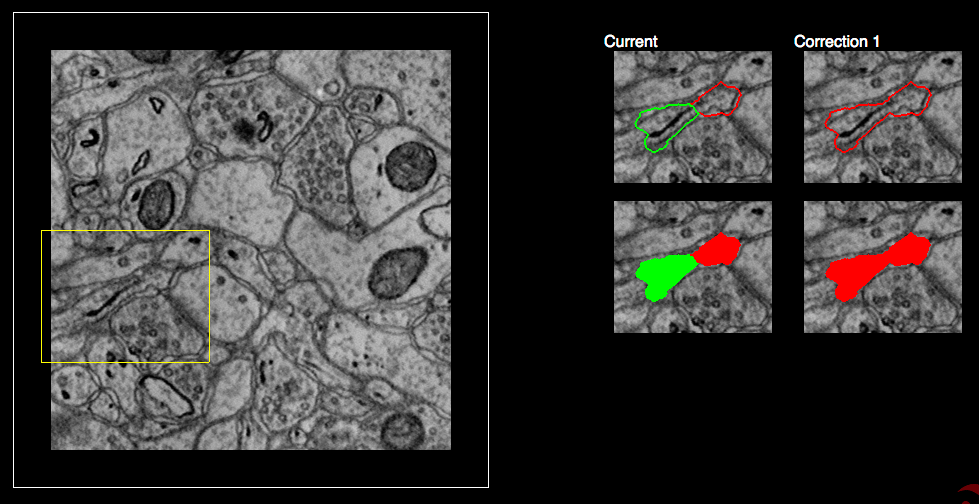
\includegraphics[width=0.95\textwidth]{gfx/proto_split.png}
    }
    \hfill
    \subfloat[Merge error]{%
      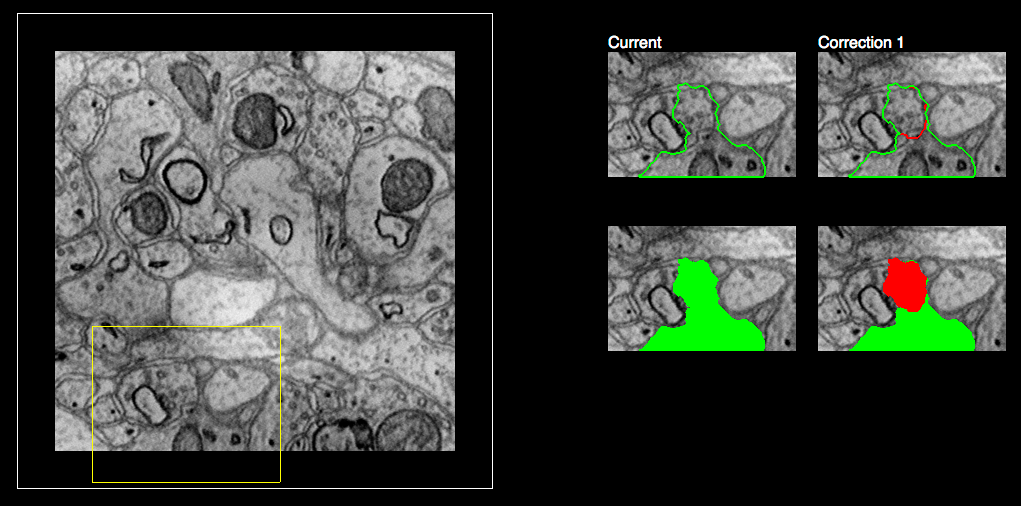
\includegraphics[width=0.95\textwidth]{gfx/proto_merge.png}
    }
	\caption{Our web-based user interface includes a slice overview with the relevant area highlighted in yellow. The interface shows (a) a split error with a suggested correction as well as (b) a merge error with correction. The user selects whether to accept a correction or to discard it.}
\label{fig:prototype}
\end{figure}
